\documentclass[11pt]{article}
\usepackage[a4paper,margin=22mm,headheight=16pt]{geometry}
\usepackage{fontspec,xeCJK,xcolor,graphicx,enumitem,fancyhdr,titlesec}
\usepackage{hyperref}
\IfFontExistsTF{Times New Roman}{\setmainfont{Times New Roman}}{\setmainfont{TeX Gyre Termes}}
\IfFontExistsTF{FangSong}{\setCJKmainfont[AutoFakeBold=2]{FangSong}}{\IfFontExistsTF{仿宋}{\setCJKmainfont[AutoFakeBold=2]{仿宋}}{\IfFontExistsTF{FandolFang-Regular.otf}{\setCJKmainfont[AutoFakeBold=2]{FandolFang-Regular.otf}}{\setCJKmainfont{FandolSong-Regular.otf}}}}
\definecolor{ink}{HTML}{173747}\definecolor{accent}{HTML}{227E82}
\hypersetup{colorlinks=true,urlcolor=accent,linkcolor=accent}
\linespread{1.22}\setlength{\parindent}{0pt}\setlength{\parskip}{6pt}
\setlist[itemize]{leftmargin=1.4em,itemsep=3pt}
\titleformat{\section}{\large\bfseries\color{ink}}{}{0pt}{}
\titlespacing*{\section}{0pt}{14pt}{7pt}
\pagestyle{fancy}\fancyhf{}\lhead{\small OMNI LEARNING / 学习手册}\rhead{\small Source-grounded learning}\cfoot{\small\thepage}
\emergencystretch=2em\widowpenalty=10000\clubpenalty=10000
\newcommand{\Needspace}[1]{\par\begingroup\dimen0=#1\relax\vskip0pt plus\dimen0\penalty-100\vskip0pt plus-\dimen0\vskip\dimen0\penalty9999\vskip-\dimen0\vskip0pt\endgroup}
\begin{document}


{\LARGE\bfseries\color{ink} 从手机看技术系统}\par

2026-10-08 | Day01/30 | 阅读 8 分钟 + 练习 3 分钟\par\vspace{6pt}

\Needspace{5\baselineskip}\section*{今日导航}

今天回答：一部手机为什么不能只用“芯片很强”来解释？学完后，你应能把熟悉的设备拆成输入、处理、输出和支撑条件，并指出一个系统瓶颈。先用一分钟回想昨天使用手机时最不顺畅的一件事。今天不用记器件型号，也不比较品牌。

\Needspace{5\baselineskip}\section*{从一个失败场景开始}

假设你在车站扫描二维码，页面迟迟打不开。第一反应可能是“手机太慢”。但相机已经识别图案，失败也可能发生在网络传输、服务器响应或身份验证。这里的场景是教学设例。分析技术的第一步，是明确任务在哪里开始、在哪里算完成，而不是立刻给某个部件下结论。

\begin{center}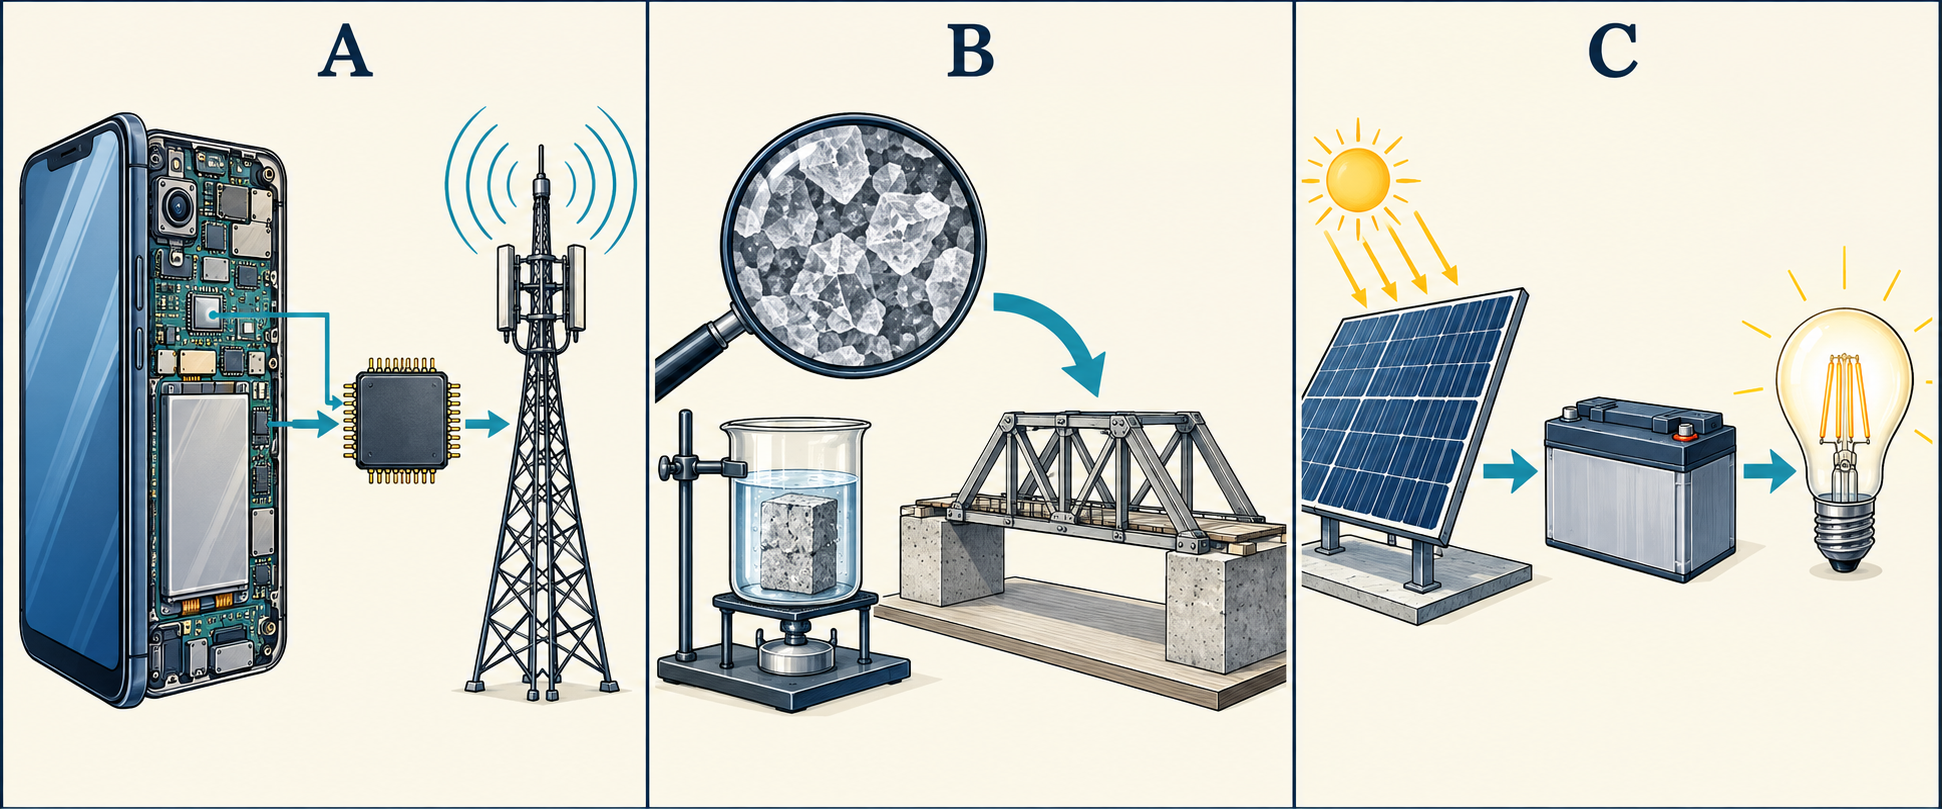
\includegraphics[width=\linewidth,height=0.26\textheight,keepaspectratio]{../assets/figure-f1c69576c177.png}\par

{\small 本课重点看 A 区。A 用手机观察部件与网络；B 区分解释与设计；C 追踪太阳能、储能和照明之间的能量流。箭头为概念关系，不是接线图。}\par

{\footnotesize AI生成教学示意，非实物照片、原始史料或官方架构。生成方式：内置文生图；提示词见仓库 docs/image-prompts.json。}\end{center}

\Needspace{5\baselineskip}\section*{核心概念：系统、接口和瓶颈}

系统是一组互相配合以完成目标的部分。手机拍照包含镜头与传感器接收光、计算处理、存储和屏幕呈现；电池为过程供能。可以先画框，再问每个框接收什么、输出什么。不同任务会改变你关心的边界：如果目标是把照片发给朋友，通信网络和对方设备也进入系统。

接口是部分之间交换信息或作用的约定。插头能接上不意味着文件能读懂，文件能打开也不意味着内容正确。硬件连接、数据格式和业务规则解决的是不同层次的问题。NASA 的波谱资料说明，无线通信与可见光同属电磁现象，但频段与用途不同，不能因为同属一种物理现象就假定能力相同。[S2]

瓶颈是当前条件下限制整体任务的环节。晶体管与集成电路的发展提供了计算能力的重要基础，但系统体验还依赖其他环节。[S5] 只有当处理能力是主要限制时，换更快的芯片才可能明显缩短等待。这不是说芯片不重要，而是先定位限制再选择改进。

\Needspace{5\baselineskip}\section*{读图与案例：扫码迟缓的排查}

看图 A，把箭头理解为部件间的联系，而非真实手机接线。请补上图中没有画出的服务器与软件。

做一个小型诊断表：相机无法对焦，对应输入环节；二维码能识别而网页打不开，对应传输或服务环节；网页已打开但无法登录，对应身份或业务环节。同一个“打不开”的感受，可能对应不同证据。每次只改变一个条件，例如换网络后重试；如果同时换设备、网络和账号，即使恢复正常，也难判断哪个因素起作用。

\Needspace{5\baselineskip}\section*{三分钟练习与自查}

选择电梯、导航或洗衣机中的一个，写下“用户目标—三个组成部分—一个接口—一个可能瓶颈”。用两分钟完成，再花一分钟自查。

参考：导航的目标是到达目的地；组成包括定位、地图与路线计算；接口包括位置数据进入路线模块；地铁内定位误差可能成为瓶颈。自查时确认你写的是可观察的问题，而非“AI不够聪明”这类不可直接验证的评价。答案不唯一，但必须能说明如何取得证据。

\Needspace{5\baselineskip}\section*{带走的判断与明日连接}

今天把技术对象从名词拆成了完成任务的系统。下次遇到“性能翻倍”的新闻，先问测的是什么任务、哪个环节、在什么条件下。NIST 对 AI 的测量工作也把可靠性等维度与准确性并列，这说明单一指标不能描述全部能力。[S4] 明天继续学习：什么样的证据能支持一个技术判断？

\Needspace{6\baselineskip}\section*{扩展学习 / Further reading}\small 以下为选读，不计入每日必做时间。\begin{enumerate}[leftmargin=1.6em]

\item [S1] \href{https://openstax.org/books/physics/pages/1-1-physics-definitions-and-applications}{Physics: Definitions and Applications} — 从物理学与技术的关系入手，区分解释自然和解决实际问题。\par OpenStax | 发布：未标注 | 核验：2026-10-08

\item [S2] \href{https://science.nasa.gov/ems/}{The Electromagnetic Spectrum} — 查看波谱教学材料，理解通信与成像共享的物理基础。\par NASA | 发布：未标注 | 核验：2026-10-08

\item [S3] \href{https://www.energy.gov/oe/electricity-101}{Electricity 101} — 只读发电、输电、配电与 kWh 的基础解释；历史统计不作当前数据。\par 美国能源部 | 发布：未标注 | 核验：2026-10-08

\item [S4] \href{https://www.nist.gov/ai-measurement-and-evaluation}{AI measurement and evaluation} — 观察准确性之外的可靠性与可解释性维度，为后续技术评估做准备。\par NIST | 发布：未标注 | 核验：2026-10-08

\item [S5] \href{https://www.computerhistory.org/siliconengine/}{The Silicon Engine} — 沿晶体管与集成电路历史观察技术如何通过多项改进进入系统。\par Computer History Museum | 发布：未标注 | 核验：2026-10-08

\end{enumerate}

\end{document}